\chapter{}
\section{Introduction}
The statement "Smartphones have revolutionised the way we shop" is one that I believe to be true, though the market and key technologies remain the need to make further advances to fulfil the claim more solidly.
The term 'revolutionised' is defined to mean the completion of a change (be that radically new or innovative) \cite{dictionary} of something to make it better. Applying this to shopping, the arguments and statistics in this paper show why smartphones have played a large role. \par
To look into further depth behind my reasons for this, this report gives an insight into how much smartphones have developed in terms of shopping support, and how they have become a more prominent force in quicker purchases, advertising and ease of use for shoppers. Social, ethical and legal issues have also been considered in my decision, looking at what restrictions shopping through a smartphone may occur compared to contemporary face to face shopping. As with any argument, an opposing opinion has also been considered, in order to back up my own personal choice by comparing the two. \par

\subsection{Smartphone statistics}

To build up a confidence in the sheer size of the smartphone market in recent times, and the increase in smartphone abilities, the following graphs show statistics from the past 5 years. Figure 1.1 shows how the smartphone is now replacing the feature phone (phones with basic call functionality).
\begin{figure}[H]
  \caption{Share of total handsets by type. Statistics from The Register (2009) \cite{register}}
  \centering
  \label{fig:feature}
    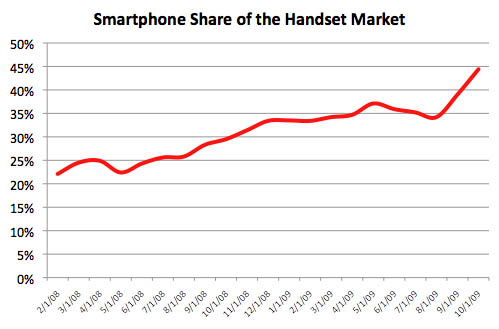
\includegraphics[width=0.5\textwidth]{stat0}
\end{figure}
Figure 1.2 shows that in addition to smartphones, the way people using them is now primarily in data, where just 7 years ago it was for calls. Figure 1.3 also shows that this is happening in every age group, with increases of more than double.

\begin{figure}[H]
\centering
\begin{minipage}{.5\textwidth}
  \centering
  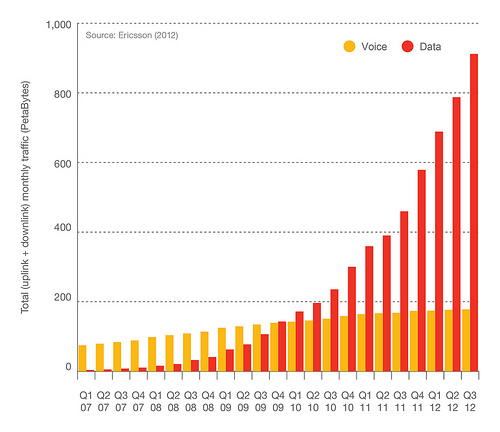
\includegraphics[width=.9\linewidth]{stat1}
  \captionof{figure}{The shift in primarily voice \\calling to data usages in mobile phones.}
  \label{fig:test1}
\end{minipage}%
\begin{minipage}{.5\textwidth}
  \centering
  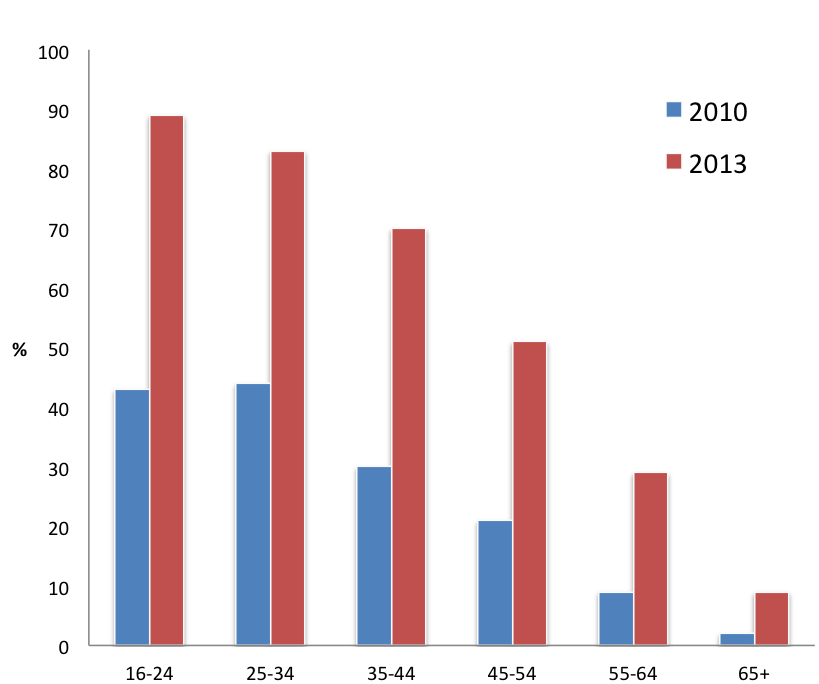
\includegraphics[width=.9\linewidth]{stat2}
  \captionof{figure}{Age groups using smartphones for data, between 2010 and 2013. Statistic from InfoDocket 2012 \cite{docket}.}
  \label{fig:test2}
\end{minipage}
\end{figure}

\section{Key technologies in the shopping market} 

Upon investigating the major advances made in the retail market since the introduction and rise of smartphones, several papers and statically reports provided useful in analysing the statement mentioned earlier. In a paper by M. K. Janiak \cite{overview}, they give a good overview of new technologies offered by the smartphone market in terms of retail experiences, and break the advances into seven main categories as shown in figure 1.4. \par
 \begin{figure}[H]
  \caption{Smartphone retail enhancements, as depicted by M Janiak \cite{overview}.}
  \centering
  \label{fig:retail}
    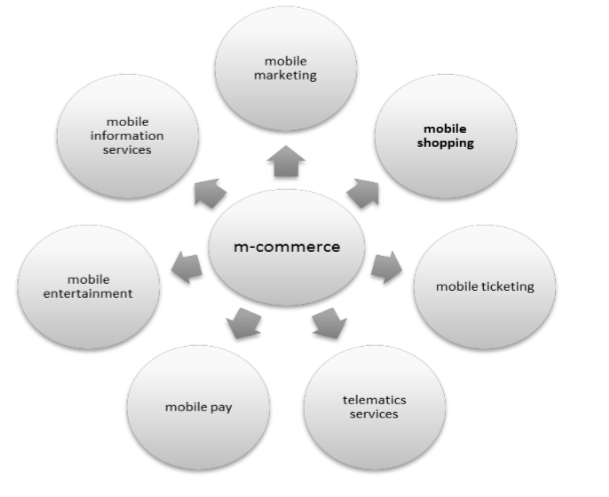
\includegraphics[width=0.5\textwidth]{retail}
\end{figure}
By having a look at some of the major categories defined in this paper, examples of these technologies will provide support for the argument that the statement is true. One clear great advantage that comes with the post 2010 era of mobile phones is the availability to pay for products in a number of retailers and food outlets directly via a phone's near-field communication functionality. \par

With application such as Apple pay and Android pay (Though this is only yet released in the US as of the time of this paper) now usable in an increasing number of businesses, consumers have gained from the speed of transactions, and the reduced need to have either cash or card on their person when shopping. Figure 1.5 shows that although this is remains in its early stages, the amount of mobile who have used mobile payments has almost doubled over the past year alone. Reasons this is only increase now is because of the reliant of the shop or service to allow users to pay via mobile. As most phones have the NFC (Near Field Communication) feature, this will only become an easier to implement system in the future.

 \begin{figure}[H]
  \caption{Apple Pay usages increase between the year 2014 and 2015. Statistics taken from Pymnts 2015 \cite{apple-pay}.}
  \centering
  \label{fig:nfc}
    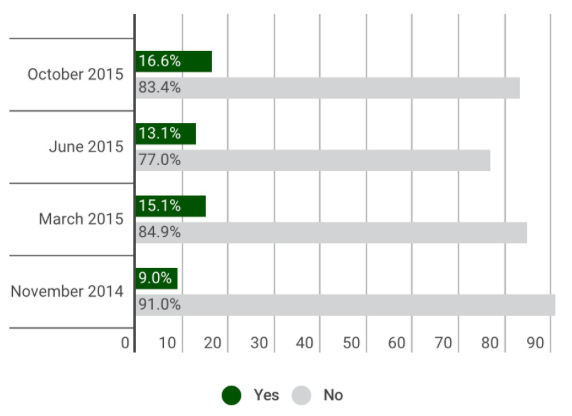
\includegraphics[width=0.6\textwidth]{nfc}
\end{figure}

Shops and services that do not allow mobile payment can however allow users to benefit from smartphones, through the ability to suit a consumer's needs, by live deals, vouchers, or simply with the option to buy online through mobile. In a paper by G. Cliquet \cite{french}, the author says that mobile web sites and apps allow the exposure of four mobile characteristics. The two most important and relevant to the revolutionary shopping experience using mobiles is 'enhanced usability', allowing a user to connect and use the Internet anywhere, whilst 'synchronicity' allows smartphones to synchronise with customers' needs and provide them with personalised options and results. \par
What this means for a user is they are provided with a means of purchase, and one that is customised for them, providing that the seller provides a basic platform. It also means that mobile websites provide this option without the need for an app. \par
In addition to having the ability to purchase everyday products through smartphones, users now have more confidence in the security of their purchases. As technology becomes more and more advanced, the protection of passwords, personal details, and payment details also become safer. With this is mind, it has contributed to the shear rise in sales via smartphones. Figure 1.6 shows the increase year on year for a range of retail companies from sales via smartphones compared to those visited on a desktop machine. Although smartphones are not leading sale amounts, the increase in sales compared to those of desktops is vastly more.
 \begin{figure}[H]
  \caption{Increase in sales for PC and desktop between 2014 and 2015. Statistics taken from D. Chaffey of Smart-insights 2015 \cite{smart-insights}.}
  \centering
  \label{fig:increase}
    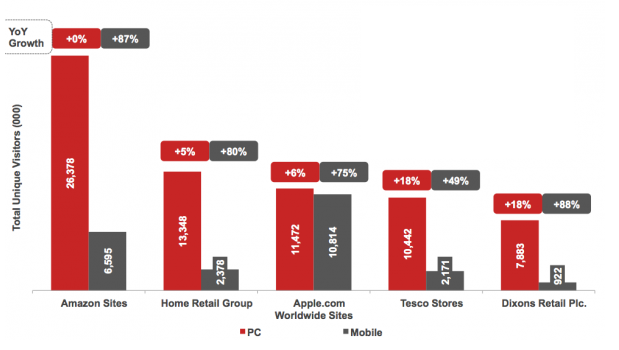
\includegraphics[width=0.6\textwidth]{increase}
\end{figure}
As Figure 1.7 shows, even when a user may not be buying directly through smartphones, they are still allowing a revolutionary change in shopping by allowing users to view products, compare and search for reviews before buying them in person. With the use of QR codes, this can speed up the shopping process even faster, by giving users the ability to access product information without having to search, or go to specific web page. QR codes have become an ever more used way of linking users to a service, due to the small size of the code, and because most users have a phone with a camera and an internet connection (as shown in the introductory part of this paper.). \par
  \begin{figure}[H]
  \caption{Percentages of use of smartphones for various retail activities for all users with smartphones. Taken from Delotte consumer survey 2013.}
  \centering
  \label{fig:delotte}
    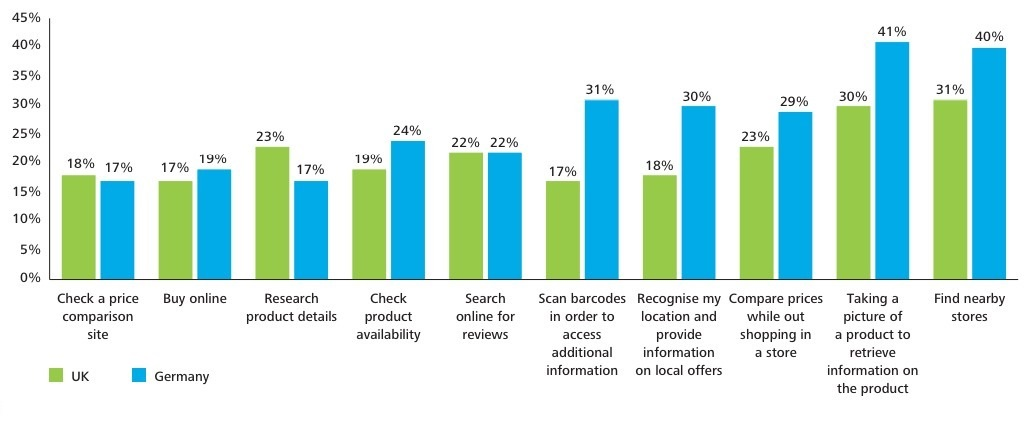
\includegraphics[width=0.9\textwidth]{usage}
\end{figure}
On top of the camera and Internet functionality that allows users to take advantage of smartphones when shopping, are a growing number of other features available to users. For example, with location services now enabled on most phones, applications are able to take advantage of this to inform the user when a nearby store has an offer, or if they are close to a store event. On the other hand, it allows users to actively seek out retailers using their position, and combined with online reviews of that retailer, they are then able to choose the most appropriate. Comparing this to the past when smartphones did not allow this, a person in this situation would rely on mouth to mouth for reviews, and the use of a directory or map to find a shop. This is one example of how simple features have made a shoppers life easier. \par

Another closely linked 'revolution' to smartphone shopping is the use of social media in everyday life. Because of the rise in people using social media, this is allowing businesses to communicate with a mass of potential customers through sites such as Facebook. In 2015, it was found that 54\% of businesses generated leads through social media \cite{business}, and reinforcing this further, it was found that in the same year 83\% (out of the 1.1 billion users) of Facebook access the service through mobile devices \cite{facebook}. This makes this means of communication very cost effective and easier than paying for more traditional advertising campaigns. \par

Another way shopping through smartphones has become a revolution is not through sales, but through the support of those sales. In past years, a user buying anything from a retailer would call the company if they found any problems with their service, but now many retailers provide online and mobile live support. From live chat, to forums, users are able to find answers on the go, and do this quickly. Last year, Amazon launched the Mayday button \cite{mayday}, allowing a user to get instant live support with video of a representative if they were either stuck with an issue from amazon products, or their smartphone directly. The customer service provided promises an answer in 15 seconds or less, and they have the ability to draw on a user's screen in informing them what they should do.

\section{Legal, social and ethical implications of key technologies}

Although smartphones have revolutionised shopping in terms of the ability to shop, the ease and the speed, the gain in smartphone use and functionality has also brought with it implications ethically and legally. One major concern with the rise in online shopping is privacy of users. When a user installs an application, or uses a site through a mobile, services such as location can be used to fetch customised deals. However, services and retailers must also be aware of privacy laws (such as the Data Protection Act 1998) which can be broken if a user is followed too much \cite{french}.  \par
By tracking a user's habits without their consent, be that the searches they have made, or products they have bought in the past, the retailer could be breaking that law. In addition to this, using a user's smartphone in ways such as spamming a user through their emails would look unethical and be an annoyance for a user (since lots of users must manually log into an app or website to disable emails for instance.). \par
This follows a similar suit for games and in-app purchases, where users may feel pressured or recommended by a game to buy add-ons, boosts or ways in which they can benefit more than normal free-to-play users. By sending a user a notification of a deal may mean impulse buying, which again is not covered by law, but can be seen as unethical by society. \par
In terms of security, this is also one of the biggest factors to look at when implementing online and particularly mobile shopping. The more users that input passwords, bank details and other personal information into mobile devices, the more it is targeted by attackers, meaning vendors must ensure they are safe to use. In the US the Computer Security Act of 1987 had the intention of setting a minimum acceptable security system for all owners, ensuring that sensitive information is safe. Even then however, attacks are reported on a daily basis, and where companies have been using weak safeguards, there has been various law suits, and exposure to the general public. \par
Although QR codes are a very useful way of reaching sites, they show one example where users may be at risk of opening unknown links, and could be susceptible to viruses. Because of the ever changing ways smartphones are used, new threats and cases of misuse will have to be judged. 

\section{Conclusion}
With the statistics and examples presented in this paper, it is clear that there is a large amount of opportunities for both sellers and buyers to make the most out of smartphones currently. Although the original statement sounds close to what has happened in current times, it can be seen that there is still some progress to be made to further be applied to a wider population. \par
In 2015, around 1.8 billion users had smartphones \cite{population}. Although this seems a lot, it means that not all the population currently have the ability to shop through their phone, or use a phone to enhance their shopping experience. It is predicted from the same source that in 2019 over 2.5 billion will have smartphones. There is still a gap between the ages of users, where younger ones feel more confident of using smartphones to purchase whilst older ones who are not as adept with the newer technology more cautious. \par
As the smartphone market expands, and newer technology is released, it is required that laws cover more and more issues, and older ones may become less required. This is similar to ethical opinions too, where something that is seen as unnecessary or not an issue may flip in the next 10 years.

Word count (excluding figure captions and bibliography): 1977.

\begin{thebibliography}{1}
  
\bibitem{dictionary}
LLC. (2016). \emph{Define Revolutionise}. \hskip 1em plus
  0.5em minus 0.4em\relax [Online]. Available: \url{http://www.dictionary.com/browse/revolutionize} (Accessed 11/05/2016).

\bibitem{register}
R.~Myslewski. (2009). \emph{iPhone conquers half the (smartphone) world}. \hskip 1em plus
  0.5em minus 0.4em\relax [Online]. Available: \url{http://www.theregister.co.uk/2009/11/24/admob_mobile_metrics_report/} (Accessed 11/05/2016).
  
\bibitem{docket}
C.~Benari. (2013). \emph{How big is the UK smartphone market?}. \hskip 1em plus
  0.5em minus 0.4em\relax [Online]. Available: \url{http://districthealth.co.uk/big-uk-smartphone-market/} (Accessed 12/05/2016).

\bibitem{overview}
M.~Kiba-Janiak. (2014). \emph{The use of mobile phones by customers in retail stores}. \hskip 1em plus
  0.5em minus 0.4em\relax [Journal]. Economics \& Sociology, Vol. 7, No 1, 2014. (Accessed 12/05/2016).

\bibitem{french}
G.~Cliquet et.al. (2014). \emph{Shopping with a Smartphone: A French-Japanese
Perspective}. \hskip 1em plus
  0.5em minus 0.4em\relax [Online]. Available: \url{http://www.igr.univ-rennes1.fr/sites/default/files/fichier-publication/Marketing\%20ZFP\%202-2014\%20Cliquet_et_al.pdf} (Accessed 13/05/2016).

\bibitem{apple-pay}
PYMNTS. (2015). \emph{Apple Pay adoption numbers}. \hskip 1em plus
  0.5em minus 0.4em\relax [Online]. Available: \url{http://www.pymnts.com/news/2015/new-apple-pay-adoption-numbers/} (Accessed 13/05/2016).

\bibitem{smart-insights}
D.~Chaffey. (2015). \emph{Mobile marketing statistics compilation}. \hskip 1em plus
  0.5em minus 0.4em\relax [Online]. Available: \url{http://www.smartinsights.com/mobile-marketing/mobile-marketing-analytics/mobile-marketing-statistics/} (Accessed 13/05/2016).

\bibitem{business}
IronPaper. (2015). \emph{Social Media Marketing Statistics for 2015}. \hskip 1em plus
  0.5em minus 0.4em\relax [Online]. Available: \url{http://www.ironpaper.com/webintel/articles/social-media-marketing-statistics-2015/} (Accessed 13/05/2016).

\bibitem{facebook}
S.~Kemp. (2015). \emph{Digital, social and mobile worldwide in 2015}. \hskip 1em plus
  0.5em minus 0.4em\relax [Online]. Available: \url{http://wearesocial.com/uk/special-reports/digital-social-mobile-worldwide-2015} (Accessed 13/05/2016).
  
\bibitem{mayday}
Amazon. (2016). \emph{Get help with Mayday}. \hskip 1em plus
  0.5em minus 0.4em\relax [Online]. Available: \url{http://www.amazon.co.uk/gp/help/customer/display.html?nodeId=201556310} (Accessed 13/05/2016).

\bibitem{population}
Statistica. (2016). \emph{Number of smartphone users worldwide from 2014 to 2019}. \hskip 1em plus
  0.5em minus 0.4em\relax [Online]. Available: \url{  
http://www.statista.com/statistics/330695/number-of-smartphone-users-worldwide/} (Accessed 13/05/2016).

\end{thebibliography}